\documentclass[a4paper, 10pt]{article}
\usepackage[margin=0.5in]{geometry}
\usepackage{comment} % enables the use of multi-line comments (\ifx \fi) 
\usepackage{lipsum} %This package just generates Lorem Ipsum filler text. 
\usepackage{fullpage} % changes the margin
\usepackage{multirow}	
\usepackage{amssymb}
\usepackage{amsmath}
\usepackage{graphicx}
\usepackage{listings}
\usepackage{hyperref}

\newcommand\tab[1][1cm]{\hspace*{#1}}
\newcommand{\norm}[1]{\left\lVert#1\right\rVert}
\newcommand{\p}[1]{\left(#1\right)}
\newcommand{\bk}[1]{\left[#1\right]}
\newcommand{\bc}[1]{ \left\{#1\right\} }
\newcommand{\abs}[1]{ \left|#1\right| }
\newcommand{\mat}{ \begin{pmatrix} }
\newcommand{\tam}{ \end{pmatrix} }
\newcommand{\suml}{ \sum_{i=1}^n }
\newcommand{\prodl}{ \prod_{i=1}^n }
\newcommand{\ds}{ \displaystyle }
\newcommand{\df}[2]{ \frac{d#1}{d#2} }
\newcommand{\ddf}[2]{ \frac{d^2#1}{d{#2}^2} }
\newcommand{\pd}[2]{ \frac{\partial#1}{\partial#2} }
\newcommand{\pdd}[2]{ \frac{\partial^2#1}{\partial{#2}^2} }
\newcommand{\N}{ \mathcal{N} }
\newcommand{\E}{ \text{E} }
\newcommand{\alphaPo}[1]{ \alpha P_0(#1) }
\newcommand{\Po}[1]{ P_0(#1) }
\newcommand{\Bi}[1]{B_#1}
\begin{document}
%Header-Make sure you update this information!!!!
\noindent
\textbf{STAT 222 Homework \#1} \hfill \textbf{Mary Silva}\\
UCSC \hfill  22 April 2020\\
\\
\begin{enumerate}
    \item[1.] 
    \begin{enumerate}
        \item[(1)] $(Y_1, ..., Y_k) \sim Dir(a_1,..., a_k)$. Consider a partition $I_1,..., I_M$ of $\{1,...,k\}$. Let $U_j = \sum_{u\in I_j} Y_i$ for $j=1,...,M$. Using the definition of the Dirichlet as independent gamma random variables, $(Y_1,..., Y_k)$ can be constructed as $\left( \frac{Z_i}{Z}, ... , \frac{Z_k}{Z}\right)$ where $Z_i \stackrel{ind}{\sim} \Gamma(a_i, 1)$ and $Z = \sum_{i=1}^k Z_i$. Then
        \begin{align*}
            (U_1, ..., U_m) &= \left( \sum_{i \in I_1} Y_i,\sum_{i \in I_1} Y_i, ..., \sum_{i \in I_M} Y_i \right)\\
            &= \frac{1}{\sum_{i=1}^k Z_i} \left(\sum_{i \in I_1} Z_i, \sum_{i \in I_2} Z_i,... \sum_{i \in I_M} Z_i \right)\\
            & \stackrel{d}{=} \frac{1}{\Gamma( \sum_{i=1}^k a_i, 1)}\left(\Gamma\left(\sum_{i\in I_1} a_i, 1\right),\Gamma\left(\sum_{i\in I_2} a_i, 1\right), ... \Gamma\left(\sum_{i\in I_M} a_i, 1\right) \right)\\
            & \stackrel{d}{=} Dir\left( \sum_{i\in I_1} a_i, \sum_{i\in I_2} a_i, ..., \sum_{i\in I_M} a_i\right)\\
            &\stackrel{d}{=} Dir(b_1, ..., b_M)
        \end{align*}
        Therefore, $(U_1,..., U_M) \sim Dir(b_1, ..., b_m)$ where $b_j = \sum_{i\in I_j} a_i$.
    \end{enumerate}
    \item[(2)] Since we just showed $U_j \sim Dir(b_j, ... , b_m)$, then $Y_i/U_j \stackrel{ind}{\sim} Dir(a_i, i\in I_J)$
    \item[(3)] I never got around to these.
    \clearpage
    \item[2.] Show that for any (measurable) disjoint subsets $B_1$ and $B_2$ of $\cal{X}$, $Corr(P(B_1), P(B_2))$ is negative. Is the negative correlation for random probabilities induced by the DP prior a restriction? Discuss.
    
    \textbf{Solution: }
    Define $B_1 \cup B_2 \cup B_3 = X$, where $B_3 = (B_1 \cup B_2)^c$. Without loss of generality, $B_1$ and $B_2$ are any measurable subset of the sample space. In order to compute the correlation, it is sufficient to show that the covariance is negative because the variance is just a positive scalar factor. 
    
    Given that $P$ is a Dirichlet process
    $$P(B_1), P(B_2), P(B_3) \sim Dir(\alphaPo{B_1}, \alphaPo{B_2}, \alphaPo{B_3})$$
    where $\alpha > 0$ and $\Po{\cdot}$ is a probability measure.
    
    The covariance is computed as $$Cov(P(\Bi{1}), P(\Bi{2}))=E[P(\Bi{1})P(\Bi{2})] - E[P(\Bi{1})]E[P(\Bi{2})]$$
    Using the definition of the Dirichlet distribution in terms of independent gamma random variables, $Z_i \sim Gamma(\alphaPo{B_i}, 1)$ and $Z \sim Gamma(\sum_{j = 1}^{k} \alphaPo{B_i},1)$. Then the expected value is defined as
    $$ E[P(\Bi{i})] = \frac{E(Z_i)}{E(Z)} = \frac{\alphaPo{B_i}}{\alphaPo{B_1} + \alphaPo{B_2} + \alphaPo{B_3}} = \frac{\alphaPo{B_i}}{\alphaPo{X}} = P_0(B_i)$$
    %We use the multivariate moment of the Dirichlet random variables formula to obtain
    We can derive the multivariate moment of the Dirichlet random variables. For simplicity of notation, let $U_i = P(B_i)$ and $v_i = P_0(B_i)$. Then we have
    \begin{align*}
        E[P(\Bi{1}) P(\Bi{2})] &= E(U_1 U_2)\\
        &= \int u_1 u_2 \frac{\Gamma(\alpha v_1 + \alpha v_2 + \alpha v_3)}
                            {\Gamma(\alpha v_1)\Gamma(\alpha v_2)\Gamma(\alpha v_3)}
                            u_1^{\alpha v_1 - 1} u_2^{\alpha v_2 - 1} u_3^{\alpha v_3 - 1}
                            ~d\mathbf u\\
        &= \ds\frac{\Gamma(\alpha v_1 +1)\Gamma(\alpha v_2 +1)}
                            {\Gamma(\alpha v_1 + \alpha v_2 + \alpha v_3 + 2)}
                            \ds\frac {\Gamma(\alpha v_1 + \alpha v_2 + \alpha v_3)}
                            {\Gamma(\alpha v_1)\Gamma(\alpha v_2)} \times\\
                            \vspace{.9em}
                        &  \times \int\frac{\Gamma(\alpha v_1 + \alpha v_2 + \alpha v_3 + 2)}
                            {\Gamma(\alpha v_1+1)\Gamma(\alpha v_2+1)\Gamma(\alpha v_3)}
                            u_1^{(\alpha v_1 + 1) - 1} u_2^{(\alpha v_2 + 1) - 1} u_3^{\alpha v_3 - 1}
                            ~d\mathbf u\\
                        &= \frac{\Gamma(\alpha v_1 +1)\Gamma(\alpha v_2 +1)}
                            {\Gamma(\alpha v_1 + \alpha v_2 + \alpha v_3 + 2)}
                            \ds\frac {\Gamma(\alpha v_1 + \alpha v_2 + \alpha v_3)}
                            {\Gamma(\alpha v_1)\Gamma(\alpha v_2)}\\
                        &= \ds\frac{\Gamma(\alpha)}{\Gamma(\alpha+2)}
                            \ds\frac{\alpha v_1\Gamma(\alpha v_1) \cdot \alpha v_2\Gamma(\alpha v_2)}
                            {\Gamma(\alpha v_1)\Gamma(\alpha v_2)}\\
                        &= \frac{\alpha v_1 v_2}{(\alpha +1)}\\
                        &= \frac{\alpha P_0(B_1) P_0(B_2)}{(\alpha +1)}
    \end{align*}
    Then 
    \begin{align*}
        Cov(P(\Bi{1}), P(\Bi{2})) &= \frac{\alpha}{\alpha+1}P_0(B_1)P_0( B_2 ) - \alphaPo{B_1} \alphaPo{B_2}\\
        &= \left( \frac{\alpha}{\alpha+1} - 1 \right) P_0(B_1) P_0(B_2) < 0
    \end{align*}
    Since $\frac{\alpha}{\alpha + 1} < 1$ given that $\alpha >0$ and $P_0(\cdot)$ is a probability measure.
    
    \item[4.] \textbf{Simulation of Dirichlet process prior realizations} Consider a $DP(\alpha, G_0)$ prior over the space of distributions (equivalently c.d.f's) $G$ on ${\rm I\!R}$, with $G_0 = N(0,1)$.
    \begin{enumerate}
        \item[(a)]  Use both Ferguson’s original definition and Sethuraman’s constructive definition to generate(multiple) prior c.d.f.  realizations from the $DP(\alpha,N(0,1))$, for different values of $\alpha$ ranging from small to large.\\\\
         I choose $\alpha$ to be $0.1$, $1$, $10$ and $100$. DP's are drawn from Ferguson's definition as well as from the constructive definition (both are comparable). Changing $\alpha$ changes the shapes of each realization of the prior distributions. As $\alpha$ increase, we see less discreteness and the distributions are more concentrated around the theoretical N(0,1) $-$ which represented by the black line. This is due to the fact that $\alpha$ represents how confident we are that the prior distribution is true. For each simulation using the DP I am generating 10 CDF, each represented with a different color.
         \begin{center}
            \begin{figure}
                \centering
                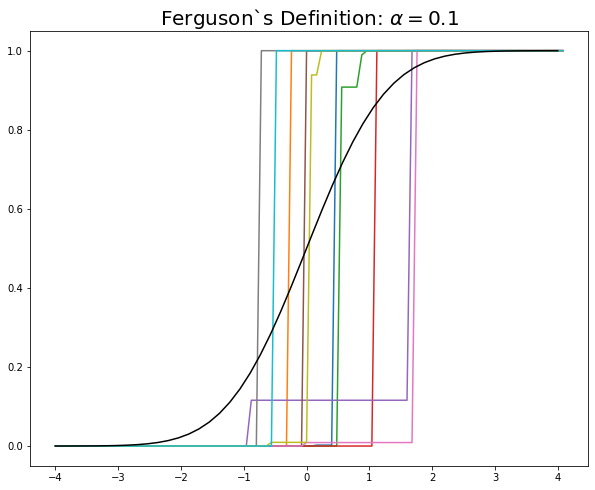
\includegraphics[scale = 0.3]{a1-1.png}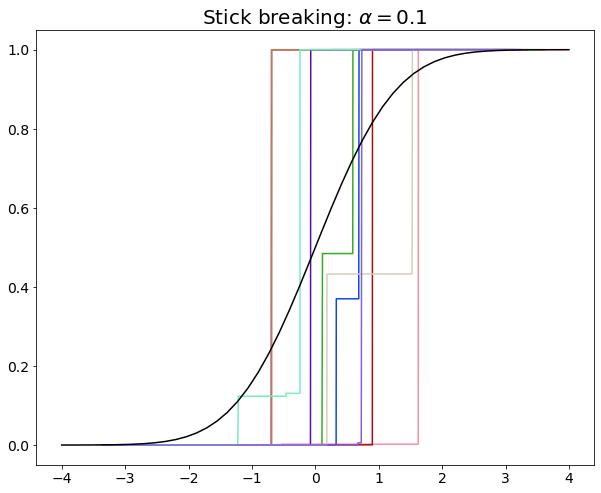
\includegraphics[scale = 0.3]{a1-5.png}
                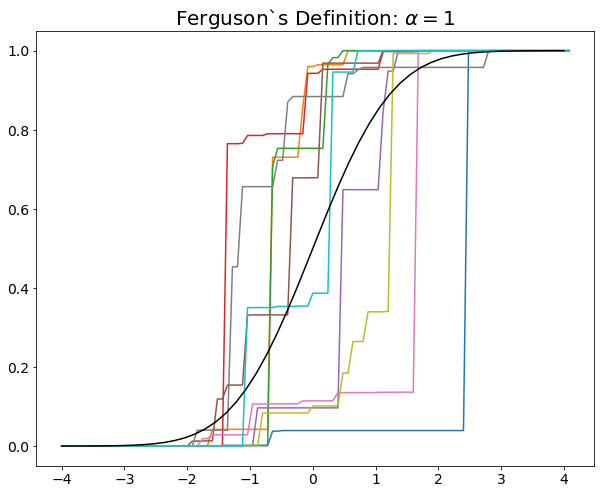
\includegraphics[scale = 0.3]{a1-2.png}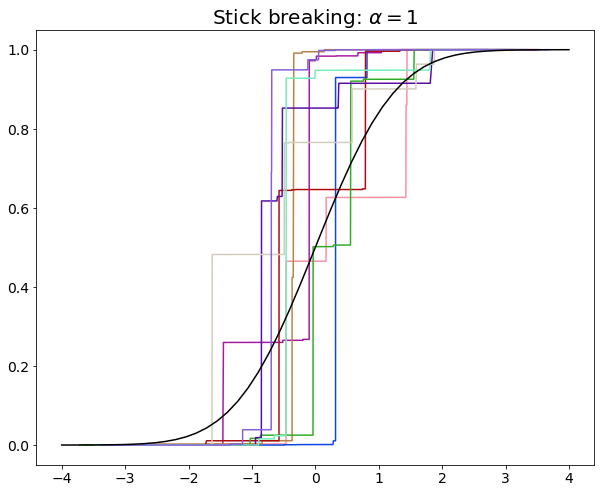
\includegraphics[scale = 0.3]{a1-6.png}
                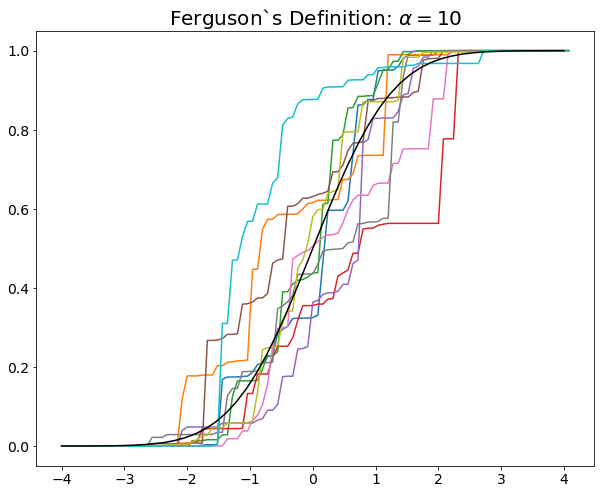
\includegraphics[scale = 0.3]{a1-3.png}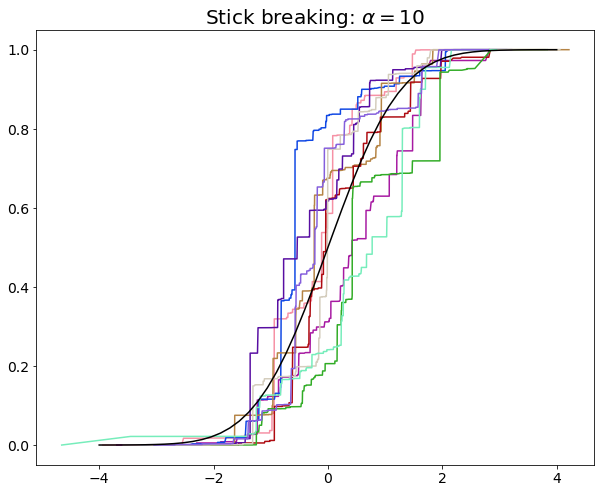
\includegraphics[scale = 0.3]{a1-7.png}
                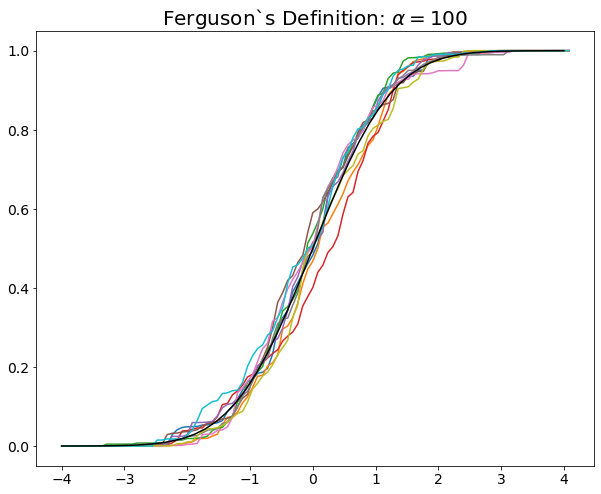
\includegraphics[scale = 0.3]{a1-4.png}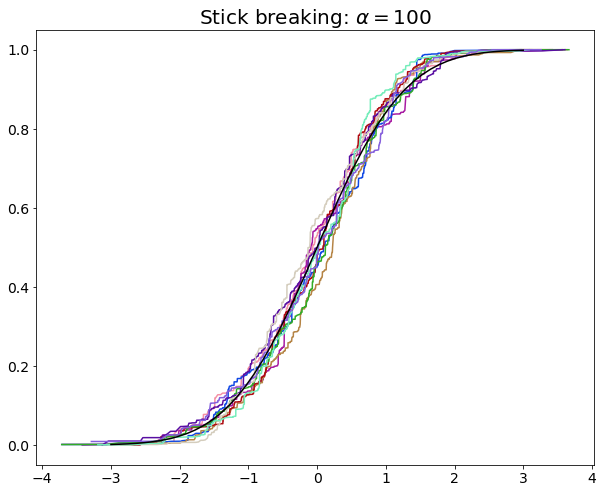
\includegraphics[scale = 0.3]{a1-8.png}
                \caption{The left plots use Ferguson’s original definition and the right plots use Sethuraman’s constructive definition with various $\alpha$. For reproducible code, see \url{https://github.com/msilva00/BNP_Homework/blob/master/HW1/HW1_Prob4.ipynb}}
                \label{part_a}
            \end{figure}
        \end{center}
        \clearpage
        \item[(b)] In addition to prior c.d.f. realizations, obtain, for each value of $\alpha$, the corresponding prior distribution for the mean functional $$\mu(G) = \int t dG(t) $$ and for the variance functional  $$\sigma^2(G) = \int t^2 dG(t) - \left\{\int t dG(t) \right\}^2$$
        
        
        \begin{center}
            \begin{figure}[h!]
                \centering
                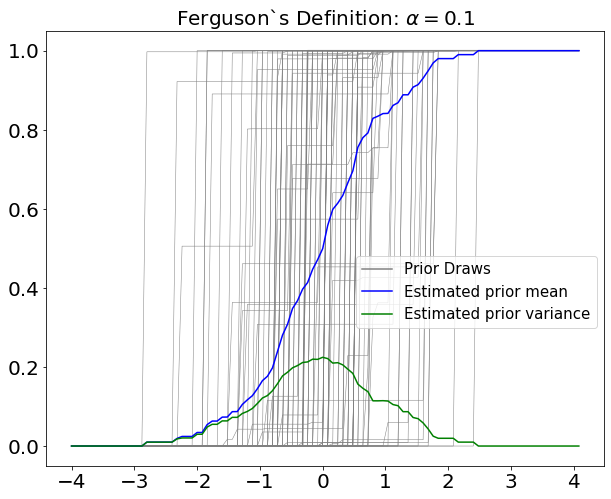
\includegraphics[scale = 0.35]{b1.png}\\
                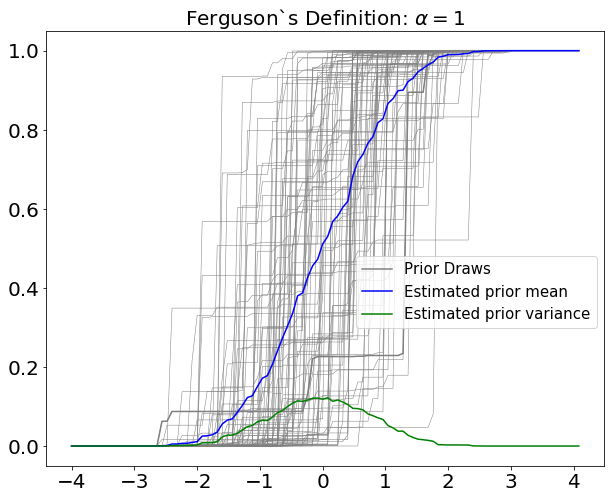
\includegraphics[scale = 0.35]{b2.png}
                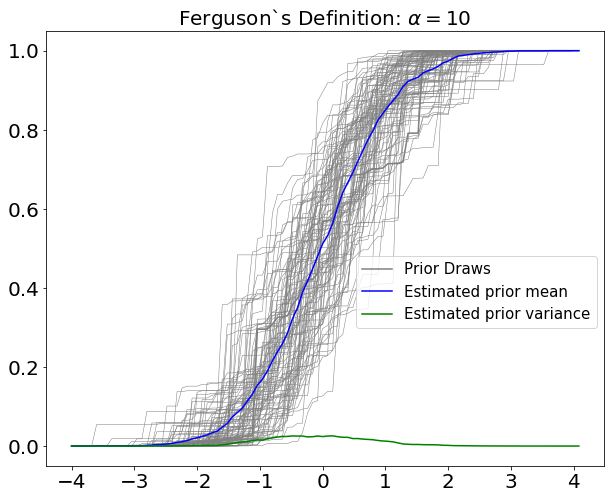
\includegraphics[scale = 0.35]{b3.png}
                \caption{Using Ferguson's definition of the DP, I can compute the functional mean and the functional variance for each simulation, fixing the value of $\alpha$. For reproducible code, see \url{https://github.com/msilva00/BNP_Homework/blob/master/HW1/HW1_Prob4.ipynb}}
                \label{part_b}
            \end{figure}
        \end{center}
        
        \item[(c)] Consider also a simulation under a mixture of DPs (MDP) prior, which extends the DP above by adding a prior for $\alpha$. Therefore, the MDP prior for G is defined such that, $G|\alpha \sim DP(\alpha, N(0,1)$, with a prior assigned to the precision parameter $\alpha$ from its prior. You can work with a gamma prior for $\alpha$ and 2-3 different choices for the gamma prior parameters.\\\\
        Next, we extend the Dirichlet process by adding a gamma prior for $\alpha$. 
        $$\alpha \sim Gamma(3,3)$$
        \begin{figure}[h!]
            \centering
            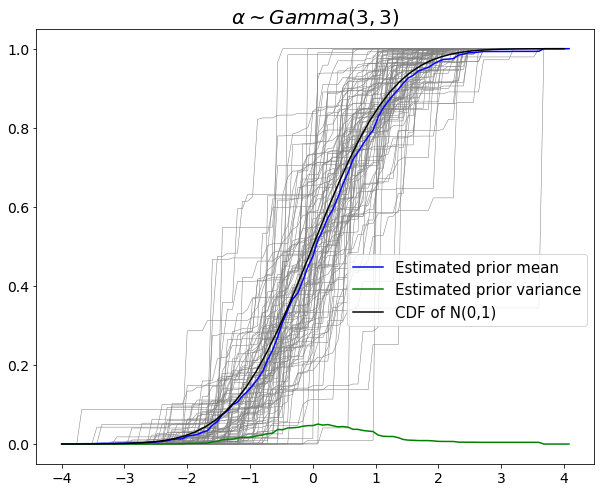
\includegraphics[scale = 0.4]{c1-1.png}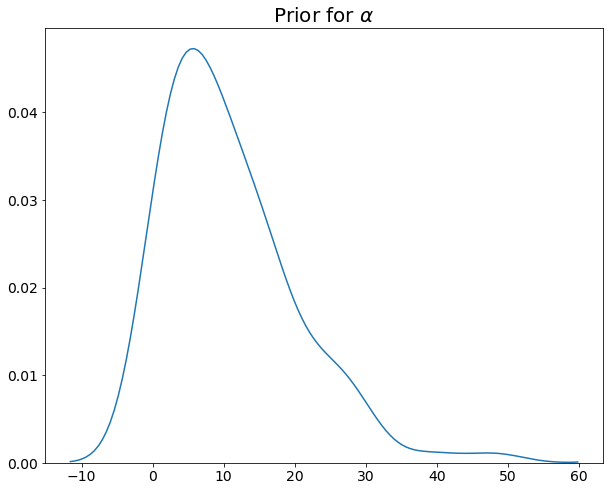
\includegraphics[scale = 0.4]{c1-2.png}
            % \caption{On the left there are results for $\alpha \sim Gamma(3,3)$. All the posterior realizations of the process are represented in violet. The mean function is plotted in blue and the red line represents the theoretical $N(0,1)$ distribution. On the left there are the results considering $M \sim Gamma(3,3)$, while on the right $M=1$. The results are very similar because the mean of the M prior distribution is close to 1. }
            \caption{Here I simulate from the MDP using Ferguson's original definition given draws for $\alpha$ from a Gamma prior. The result considering $\alpha \sim Gamma(3,3)$ is similar to the result in part a, when $\alpha = 1$ because the mean of the $\alpha$ prior distribution is close to 1.}
            \label{c1}
        \end{figure}
        
        \noindent Last, consider the following Gamma prior
        $$ \alpha \sim Gamma(1,10)$$
        \begin{figure}[h!]
            \centering
            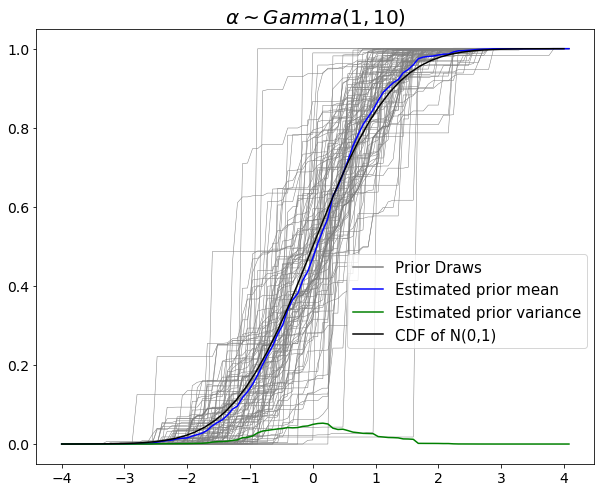
\includegraphics[scale = 0.4]{c2-1.png}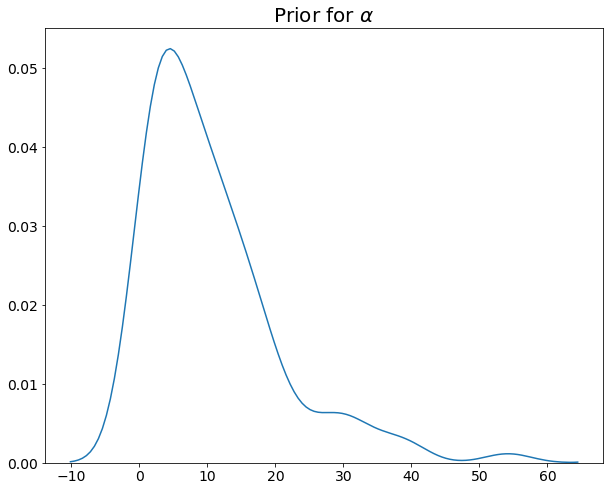
\includegraphics[scale = 0.4]{c2-2.png}
            \caption{Here I simulate from the MDP using Ferguson's original definition given draws for $\alpha$ from a Gamma prior. The result considering $\alpha \sim Gamma(1,10)$ has low variance and also small mean, putting heavy emphasis on highly discrete DP draws.}
            \label{c1}
        \end{figure}
    \end{enumerate}
\end{enumerate}
\end{document}